\subsection{A mode ladder, edge failures, and a symmetric root pencil}
\label{ssec:mode-ladder-pencil}

The next experiment fixes $C=250$ and independently assembles the finite
matrix before computing states at $N=750,1000,1250,1500$. It therefore
tests mode resolution without varying the cutoff. Matrix coefficients
use 2500 decimal digits with interval remainder bounds, and the point
Schur iteration uses 2200 digits with a fixed relative-correction stop.
The first 1000 reference windows are all requested. Reference ordinates
enter root acquisition and scoring, but not matrix assembly or the
eigenvalue computation. Every failed acquisition and every isolated
match beyond the complete prefix remains recorded.

\paragraph{Counted point-state results.}
Exact integer-polynomial sign variations bound the number of roots
below each prefix endpoint; disjoint interval-Newton enclosures supply
the matching lower count. These counts concern the newly serialized
decimal state. The first failed window contains no movable polynomial
root at $N=750$ or $1000$, as proved by a separate exact count. Carrier
zeros are counted separately. The following scores use only the complete
matched prefix and the previously fixed nearest-three-root predictor.
\begin{center}\small
\begin{tabular}{r|rrr}
$N$&Complete prefix&Within $1\%$&Worst relative prediction error\\
\hline
750&578&571/578&$2.43679$\\
1000&797&792/797&$0.707276$\\
1250&1000&1000/1000&$1.91481\cdot10^{-5}$\\
1500&1000&1000/1000&$1.69115\cdot10^{-7}$
\end{tabular}
\end{center}
The $N=1500$ run independently reproduces the earlier retained-state
maximum prediction error. At $N=1250$, the first and thousandth zeros
have respectively $1091.30879$ and $70.32801$ relative decimal digits.
At $N=1500$ they have $1175.3987$ and $305.8987$. Thus the extra 250 modes
gain about 84.09 digits at the first zero but 235.57 at the thousandth,
while $-\log_{10}\varepsilon_N$ gains only 84.09. A common eigenvalue
scale with an $N$-independent height correction cannot explain this
ladder. The mode and index dependence must interact.

\paragraph{Existence does not ensure predictor accuracy.}
At $N=750$, the first failed prediction is $k=572$, although its zero
has 6.59871 relative digits and lies in its proper window. The linear
predictor has the wrong sign. A nonlinear local solve improves the
relative error to $-1.95771\%$, still outside the gate. At $N=1000$,
the first failed prediction is $k=793$; the nonlinear error is
$+3.17251\%$. Taylor orders 16 and 24 give the same conclusions.
Other failures include wrong signs and two unsuccessful local-domain
solves. Convergence of the model solver is not convergence to the true
displacement.

An exploratory, predeclared degree ladder $p=2,3,4,6,8$ uses the same
polynomial-reproduction identity, with no fitted coefficients. For
nearest-root stencils, degree eight reduces the worst error to
$2.842\cdot10^{-12}$ at $N=1250$ and $1.196\cdot10^{-20}$ at $N=1500$.
Every target in those two prefixes passes at every tested degree.
It does not repair the lower-mode edges: degree eight passes only
568/578 and 791/797 targets at $N=750,1000$. Predecessor-only stencils
also leave failures. These exploratory successes do not replace the
original primary rule or establish a uniform remainder estimate.

\paragraph{Finite source qualification.}
A backward-error construction now certifies positivity of each
noncentral block. Exact rounded final generators and positive pivots
define a surrogate $\widehat B=L\operatorname{diag}(p)L^T>0$.
Structured interval recurrences enclose its generators, diagonal and
inverse trace. For the actual analytic block at point shift $z$,
\[
 E=\max_i\sum_j|\widehat B_{ij}-(B-zI)_{ij}|,\qquad
 g=1/\overline{\operatorname{tr}(\widehat B^{-1})}-E>0
\]
proves $B-zI\succeq gI$. This follows from the inverse-trace bound and
the symmetric row-norm perturbation bound. The exact construction,
including perturbed-generator fixtures, passes 1413 rational component
checks jointly with the pencil identities below. An initial 3200-digit
verification at $N=1500$ is too wide and is retained as a failure;
4500 verification digits succeed without changing its point state.

The independently enclosed full residual, divided by the vector norm,
is $\eta$. If its eigenvalue inclusion about $z$ lies below $z+g$,
principal-block interlacing identifies a unique simple ground eigenvalue.
The new ladder has certified relative eigenvalue radii below
$5.04\cdot10^{-166}$, $1.81\cdot10^{-172}$,
$5.31\cdot10^{-178}$ and $2.45\cdot10^{-182}$, respectively.
The generic unit-vector error bounds range from $2.60\cdot10^{-176}$
to $1.03\cdot10^{-193}$. They do not by themselves transfer every tiny
point-state displacement to the exact ground transform; indexed dual
or local root enclosures remain necessary. Increasing the $N=1000$
point arithmetic from 2200 to 2600 digits changes its eigenvalue by
less than $7.13\cdot10^{-1217}$ relatively, but leaves the shared
finite Newton stopping error. Arithmetic stability is a separate check.

\begin{proposition}[Symmetric pencil for movable squared frequencies]
\label{prop:movable-symmetric-pencil}
Write the finite even matrix as $A=\left(\begin{smallmatrix}a&c^T\\c&B\end{smallmatrix}\right)$,
with $D=\operatorname{diag}(j^2)$, $c=D^{-1}r$ and
$[D,B]=rw^T-wr^T$. Let its exact ground vector be central-normalized
as $(1,v)$ with eigenvalue $\varepsilon$, and suppose
$B_\varepsilon=B-\varepsilon I>0$ and $1+w^Tv\ne0$.
Define
\begin{align}
 H&=B_\varepsilon-cw^T-wc^T+(a-\varepsilon)ww^T,
 \label{eq:movable-pencil-H}\\
 T&=B_\varepsilon D-wr^T=DB_\varepsilon-rw^T.
 \label{eq:movable-pencil-T}
\end{align}
Then $H>0$, $T$ is symmetric, and their generalized eigenvalues are
the movable squared-frequency roots $t=(\nu/\beta)^2$, counted with
multiplicity. Hence all such squared roots are real. They are positive
if the odd parity block satisfies $A_{\rm odd}-\varepsilon I>0$.
\end{proposition}
\begin{proof}
Set $U=I+vw^T$. The eigen-equations give $B_\varepsilon v=-c$ and
$v^TB_\varepsilon v=a-\varepsilon$, so $H=U^TB_\varepsilon U>0$.
Moreover $HU^{-1}D=B_\varepsilon D-wr^T=T$, and the displacement
identity makes $T$ symmetric. The determinant lemma gives
\[
 \det(D-tU)=\det(D-tI)
       [1-tw^T(D-tI)^{-1}v].
\]
This is the movable polynomial up to a nonzero scalar, including the
lattice by polynomial continuation. The matrix $U^{-1}D$ is similar
to the real symmetric $H^{-1/2}TH^{-1/2}$. Finally, the CCM parity
formulas give $T=D^{1/2}(A_{\rm odd}-\varepsilon I)D^{1/2}$, proving
the last assertion.
\end{proof}

The pencil depends explicitly on the finite matrix and its ground
eigenvalue; its vector cancels. Under the stated positivity hypotheses,
its ordered roots satisfy the exact min--max formula
\[
 t_k=\min_{\dim V=k}\max_{0\ne x\in V}\frac{x^TTx}{x^THx}.
\]
This supplies a route to parameter-dependent resolution estimates.
Evaluating the full pencil is still a spectral computation, not the
desired input-only law. The exceptional case $1+w^Tv=0$, root
multiplicity, and matching to zeta windows require separate treatment.
For approximate states, residual corrections cannot be omitted.

The requested minimum budget must therefore be accompanied by an
indexed admissibility condition controlling the target branch, its
neighbors, and the transfer remainder. A missing branch is not a
zero-digit prediction. Uniform estimates in $C,N,k$, together with a
verified implementation residual as a function of $P$, remain the
missing steps toward a full convergence law for indices 1--1000.

\begin{figure}[htbp]
\centering
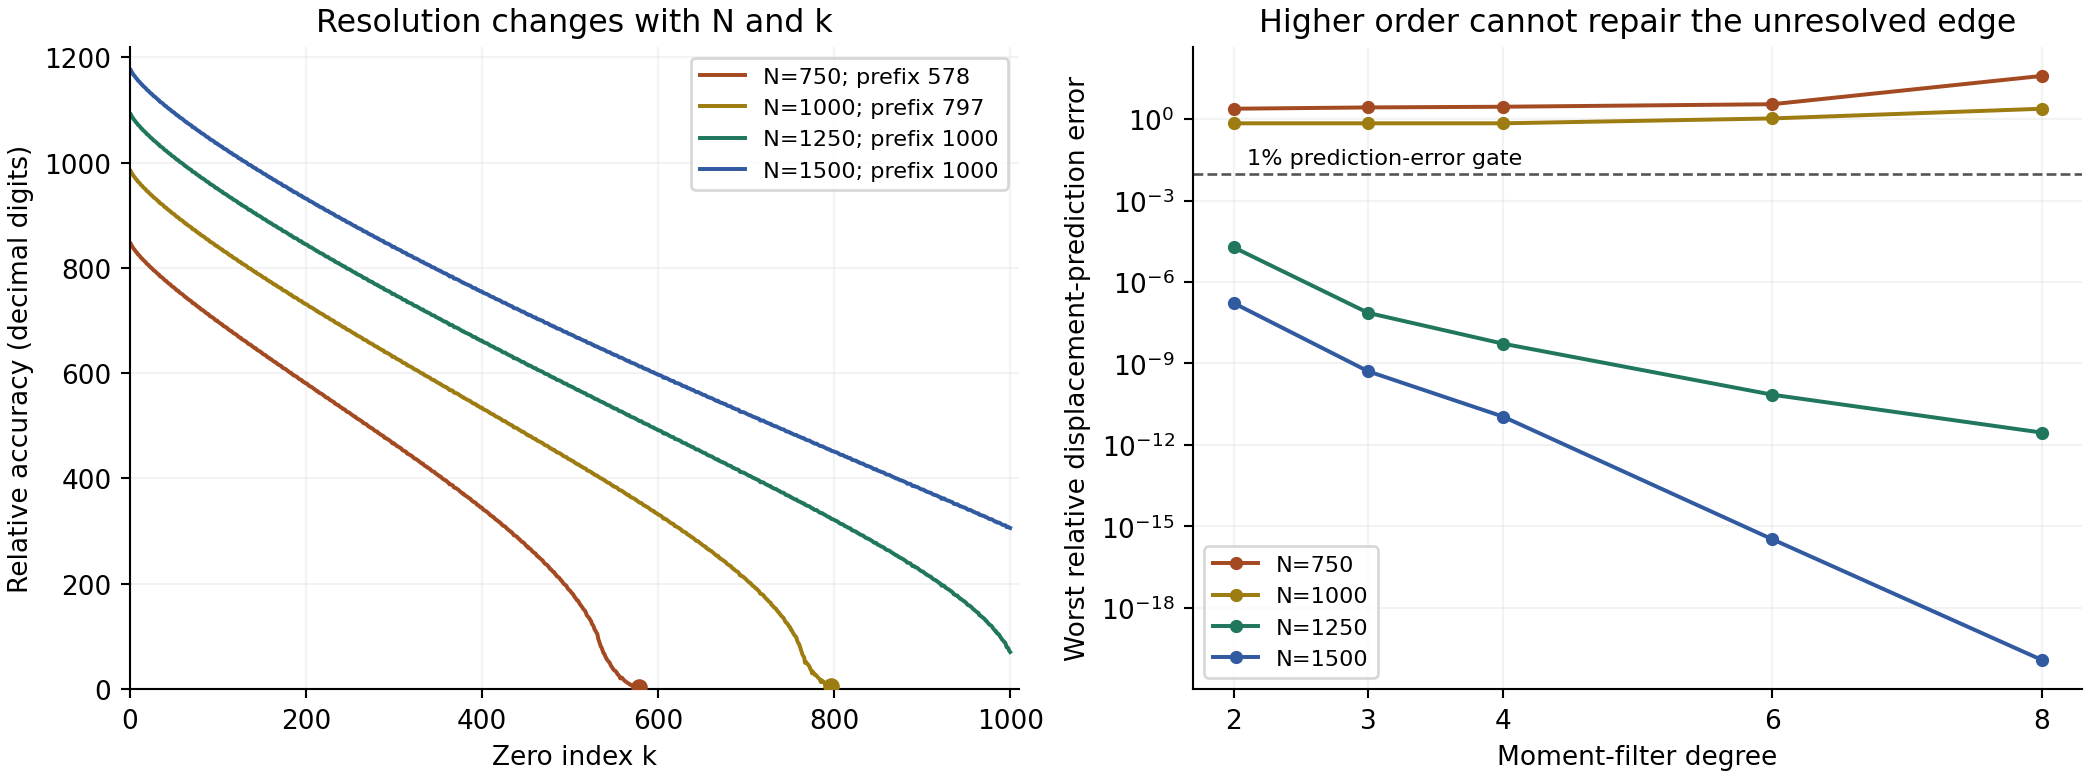
\includegraphics[width=\textwidth]{figures/mode_ladder.png}
\caption{The fixed-$C=250$ mode ladder. Left: all counted matched-prefix
point-state depths, with no continuation through absent windows. Right:
the full-prefix worst prediction error at each predeclared filter degree.
Higher order sharply improves the two well-resolved thousand-root runs
but leaves the lower-mode edge failures. Finite ground-eigenvalue
certificates and point-state root certificates have distinct scopes.}
\label{fig:mode-ladder}
\end{figure}
